%% History:
% Pavel Tvrdik (26.12.2004)
%  + initial version for PhD Report
%
% Daniel Sykora (27.01.2005)
%
% Michal Valenta (3.12.2008)
% rada zmen ve~formatovani (diky M. Duškovi, J. Holubovi a~J. Žďárkovi)
% sjednoceni zdrojoveho kodu pro~anglickou, ceskou, bakalarskou a~diplomovou praci

% One-page layout: (proof-)reading on displa
%%%% \documentclass[11pt,oneside,a4paper]{book}
% Two-page layout: final printing
%\documentclass[11pt,twoside,a4paper]{book}   
\documentclass{article}
\clubpenalty 10000
\widowpenalty 10000
\usepackage{graphicx}



%=-=-=-=-=-=-=-=-=-=-=-=--=%
% The user of this template may find useful to have an alternative to these 
% officially suggested packages:
\usepackage[czech, english]{babel}
%\usepackage[T1]{fontenc} % pouzije EC fonty 
% pripadne pisete-li cesky, pak lze zkusit take:
\usepackage[T1]{fontenc}
\usepackage{lmodern}
%\usepackage[cp1250]{inputenc}
\usepackage[utf8x]{inputenc}

\usepackage{listings}
\lstset{
  literate={ě}{{\v{e}}}1
           {š}{{\v{s}}}1
           {č}{{\v{c}}}1
           {ř}{{\v{r}}}1
           {ž}{{\v{z}}}1
           {ý}{{\'y}}1
           {á}{{\'a}}1
           {í}{{\'i}}1
           {é}{{\'e}}1
           {ó}{{\'o}}1
}


% Pozicovani
\usepackage{float}
\restylefloat{table}

%=-=-=-=-=-=-=-=-=-=-=-=--=%
% In case of problems with PDF fonts, one may try to uncomment this line:
%\usepackage{lmodern}
%=-=-=-=-=-=-=-=-=-=-=-=--=%
%=-=-=-=-=-=-=-=-=-=-=-=--=%
% Depending on your particular TeX distribution and version of conversion tools 
% (dvips/dvipdf/ps2pdf), some (advanced | desperate) users may prefer to use 
% different settings.
% Please uncomment the following style and use your CSLaTeX (cslatex/pdfcslatex) 
% to process your work. Note however, this file is in UTF-8 and a~conversion to 
% your native encoding may be required. Some settings below depend on babel 
% macros and should also be modified. See \selectlanguage \iflanguage.
%\usepackage{czech}  %%%%%\usepackage[T1]{czech} %%%%[IL2] [T1] [OT1]
%=-=-=-=-=-=-=-=-=-=-=-=--=%

%%%%%%%%%%%%%%%%%%%%%%%%%%%%%%%%%%%%%%%
% Styles required in your work follow %
%%%%%%%%%%%%%%%%%%%%%%%%%%%%%%%%%%%%%%%
\usepackage{graphicx}
%\usepackage{indentfirst} %1. odstavec jako v~cestine.

\usepackage{k336_thesis_macros} % specialni makra pro~formatovani DP a~BP



% Extension posted by Petr Dlouhy in order for better sources reference (\cite{} command) especially in Czech.
% April 2010
% See comment over \thebibliography command for details.

\usepackage[square, numbers]{natbib}             % sazba pouzite literatury
%\DeclareUrlCommandDostupné z \url{\def\UrlLeft{<}\def\UrlRight{>}\urlstyle{tt}}  %rm/sf/tt
%\renewcommand{\emph}[1]{\textsl{#1}}    % melo by byt kurziva nebo sklonene,
%\let\oldUrl\url
%\renewcommand\url[1]{<\texttt{\oldUrl{#1}}>}


\usepackage{fancyhdr}

\begin{document}
\selectlanguage{czech} 
\title{Použití jazyka CQML}
\date{}
\maketitle


\section{\label{CH:APF}Syntaxe jazyka \textit{CQML}}
V této kapitole je na příkadech vysvětlena syntaxe jazyka \textit{CQML} pro tvorbu \textit{GUI}.

\subsection{Tvorba elementů}
Kód \ref{lst:synt1} vytvoří hierarchii elementů, kde se na vrcholu nachází element základního typu \textit{Element} a v něm se nachází dva elementy typu \textit{Rectangle}, z nichž jeden obsahuje element typu \textit{MouseArea}.
\begin{lstlisting}[frame=single,caption=Syntaxe pro tvorbu hierarchie elementů.,label=lst:synt1]
Element
{
	Rectangle
	{
	};
	Rectangle
	{
		MouseArea
		{
		};
	};
}
\end{lstlisting}

\subsection{Přiřazení hodnoty atributu}
Kód \ref{lst:synt2} ukazuje nastavení hodnoty atributu \textit{width} pomocí výrazu a hodnotu atributu \textit{height} pomocí funkce vracející požadovanou hodnotu.
\begin{lstlisting}[float,frame=single,caption=Syntaxe přiřazení hodnoty elementu pomocí výrazu nebo funkce.,label=lst:synt2]
Element
{
	width : 500;
	height  : {
		return 500;
	};
}
\end{lstlisting}

\subsection{Provázání atributů}
Kód \ref{lst:synt3} demonstruje možnost provázat mezi sebou jednotlivé atributy. Vrchní element má nastavenou hodnotu atributu \textit{width} na $500$, s tímto atributem je následně provázán atribut \textit{height}, který se nastaví na hodnotu o $100$ větší. Paremetry elementu \textit{Rectangle} jsou pak provázány s hodnotami atributů nadřazeného elementu pomocí klíčového slova \textit{parent}. Tudíž oba elementy mají schodné hodnoty atributů \textit{width} a \textit{height}.
\begin{lstlisting}[frame=single,caption=Ukázka provázání atributů mezi sebou.,label=lst:synt3]
Element
{
	width : 500;
	height  : width+100;
	Rectangle
	{
		width : parent.width;
		height : parent.height;
	};
}
\end{lstlisting}


\subsection{Použití identifikátoru pro přístup k elementu}
Prostřednictvím atributu \textit{id} je možné označit element identifikátorem, pomocí něhož je možné k elementu přistupovat v rámci daného \textit{CQML} souboru. V kódu \ref{lst:synt4} je jednomu z~elementů přiřazen identifkátor \textit{firstRectangle}. Prostřednictvím tohoto identifikátoru je pak hodnota atributu \textit{width} označeného elementu přiřazena jinému.
\begin{lstlisting}[float,frame=single,caption=Ukázka přístupu k elementu a jeho atributům pomocí identifikátoru.,label=lst:synt4]
Element
{
	Rectangle
	{
		id : firstRectangle;
		width : 500;
	};
	Rectangle
	{
		width : firstRectangle.width;
	};
}
\end{lstlisting}



\subsection{Rozšíření elementu o nový atribut}
Kód \ref{lst:synt5} ukazuje rozšíření elementu o nový atribut jménem \textit{alpha} typu \textit{int} pomocí klíčového slova \textit{property}, přičemž je mu přiřazena hodnota $100$.
\begin{lstlisting}[float,frame=single,caption=Syntaxe rozšíření elementu o nový atribut.,label=lst:synt5]
Element
{
	property int alpha : 100;
}
\end{lstlisting}


\subsection{Reference na element}
V kódu \ref{lst:synt6} je kořenový element rozšířen o atribut \textit{refElement}, v němž se uchovává reference na atribut označený identifikátorem \textit{firstRectangle}. Následně je přistupováno k~atributu \textit{width} referencovaného elementu prostřednictvím dané reference.
\begin{lstlisting}[float,frame=single,caption=Ukázka přístupu k atributům elementu pomocí reference.,label=lst:synt6]
Element
{
	property Element refElement : firstRectangle;
	width : refElement.width;
	Rectangle
	{
		id : firstRectangle;
		width: 500;
	};
}
\end{lstlisting}

\subsection{Zpracování událostí}
Kód \ref{lst:synt7} ilustruje přiřazení funkce pro obsluhu události kliknutí myši. V tomto případě se po kliknutí myši na element \textit{MouseArea} změní hodnoty jeho atributů \textit{width} a \textit{height} ze~$100$ na $500$.
\begin{lstlisting}[float,frame=single,caption=Syntaxe přiřazení funkce pro obsluhu události.,label=lst:synt7]
Element
{
	MouseArea
	{
		width : 100;
		height : 100;
		MouseClicked : {
			width = 500;
			height = 500;
		};
	};
}
\end{lstlisting}

\subsection{Použití externí logiky}
Pro použití externí logiky definované v rámci uživatelské aplikace lze do kódu vygenerovaného překladačem zahrnout hlavičkový soubor pomocí příkazu \textit{include}. Kód \ref{lst:synt8} ukazuje použití funkce \textit{GetWidth}, která je deklarovaná uvnitř importovaného souboru \uv{logic.h}.
\begin{lstlisting}[frame=single,caption=Ukázka kódu používajícího externí funkci deklarovanou v hlavičkovém souboru.,label=lst:synt8]
include "logic.h"
Element
{
	Rectangle
	{
		width : {
			return GetWidth();
		};
	};
}
\end{lstlisting}


\subsection{Použití komponenty}
Samostatné soubory v jazyce \textit{CQML} lze používat jako samostatné komponenty v rámci jiných \textit{CQML} souborů, s nimiž je možno manipulovat jako s jakýmkoli jiným elementem. Toto je demonstrováno v ukázce kódu \ref{lst:synt10}, kde je pomocí příkazu \textit{import} načtena komponenta definovaná v souboru \uv{compontent1.h} (viz. kód \ref{lst:synt9}), která je pro použití označena klíčovým slovem \textit{Square}. Pomocí daného klíčového slova jsou pak vytvořeny dvě instance dané komponenty a to stejným způsobem, jako by tomu bylo u běžných elementů.
\begin{lstlisting}[float,frame=single,caption=Zdrojový soubor komponenty.,label=lst:synt9]
Rectangle
{
	property int status : 0;
	width: 500;
	height: 500;
}
\end{lstlisting}


\begin{lstlisting}[frame=single,caption=Ukázka použití komponenty z jiného souboru.,label=lst:synt10]
import "component1.h" as Square
Element
{
	width : 500;
	height : 500;
	Square
	{
		width : 100;
		height : 100;
	};
	Square
	{
		width : 200;
		height : 200;
	};
}
\end{lstlisting}



\section[Datové typy \textit{CQML}]{\label{CH:APC}Datové typy poskytované jazykem \textit{CQML}}
Knihovna \textit{CQML} poskytuje několik hodnotových a referenčních datových typů pro použití při tvorbě \textit{GUI}. Pro reprezentaci grafických elementů slouží referenční typy, aby se~například při přiřazení elementu do nějaké proměnné element nekopíroval a bylo možné s~ním manipulovat i prostřednictvím dané proměnné.
\subsection{\textit{Grafické elementy}}
Grafické elementy jsou základními stavebními souřástmi \textit{GUI} a každý z nich může být umístěn v hierarchii. Ke všem z nich je v rámci jazyka \textit{CQML} přistupováno jako k referenčním typům.

\subsubsection{\textit{Element}}
Jedná se o základní element pro použití uvnitř hierarchie \textit{GUI}. Sám nemá žádnou grafickou podobu a využívá se zejména jako kontejner pro umístění dalších grafických elementů.\\
\begin{description}
\item[Seznam atributů:] ~
\begin{description}
\item[x] - horizontální souřadnice elementu. (typ \textit{int})
\item[y] - vertikální souřadnice elementu. (typ \textit{int})
\item[width] - šířka elementu. (typ \textit{int})
\item[height] - výška elementu. (typ \textit{int})
\item[visible] - hodnota $1$ znamená, že se element vykreslí. Hodnota $0$ zamezí jeho vykreslování. (typ \textit{int})
\item[enabled] - hodnota $1$ udává, že je element zapnutý a bude reagovat. Hodnota $0$ element vypne. (typ \textit{int})
\end{description}
\item
\item[Seznam funkcí pro obsluhu událostí:] ~
\begin{description}
\item[KeyPressed] - funkce pro obsluhu stisknutí klávesy.
\item[KeyReleased] - funkce pro obsluhu puštení klávesy.
\end{description}
\end{description}


\subsubsection{\textit{Rectangle}}
Jednoduchý grafický element sloužící pro vykreslení jednoduchého obdélníku o specifikovaných rozměrech. Lze mu nastavit barvu a šířku okraje a také barvu výplně.\\
\begin{description}
\item[Seznam atributů:] ~
\begin{description}
\item[border] - šířka okraje. (typ \textit{float})
\item[borderColor] - barva okraje. (typ \textit{Color})
\item[color] - barva výplně. (typ \textit{Color})
\item[všechny atributy z typu \textit{Element}]
\end{description}
\item[Seznam funkcí pro obsluhu událostí:] ~
\begin{description}
\item[všechny funkce z typu \textit{Element}]
\end{description}
\end{description}

\subsubsection{\textit{MouseArea}}
Podobně jako základní typ \textit{Element}, nemá tento element žádnou grafickou podobu. Slouží zejména k obsluze vstupních událostí vyvolaných pomocí myši.\\
\begin{description}
\item[Seznam atributů:] ~
\begin{description}
\item[všechny atributy z typu \textit{Element}]
\end{description}
\item[Seznam funkcí pro obsluhu událostí:] ~
\begin{description}
\item[MousePressed] - funkce pro obsluhu stisknutí tlačítka myši.
\item[MouseReleased] - funkce pro obsluhu puštění tlačítka myši.
\item[MouseClicked] - funkce pro obsluhu kliknutí tlačítkem myši.
\item[MouseEntered] - funkce pro obsluhu najetí myši na plochu vymezenou elementem.
\item[MouseExited] - funkce pro obsluhu vyjetí myši z plochy vymezené elementem.
\item[MouseMoved] - funkce pro obsluhu pohybu myši.
\item[MouseScrolled] - funkce pro obsluhu otočení kolečkem myši.
\item[všechny funkce z typu \textit{Element}]
\end{description}
\end{description}

\subsubsection{\textit{Image}}
Grafický element sloužící pro zobrazení obrázku načteného ze souboru. V případě, že rozměry obrázku v souboru jsou odlišné od rozměrů elementu, pak se obrázek roztáhne či smrští do definované plochy.\\
\begin{description}
\item[Seznam atributů:] ~
\begin{description}
\item[img] - data obrázku. (typ \textit{Img})
\item[všechny atributy z typu \textit{Element}]
\end{description}
\item[Seznam funkcí pro obsluhu událostí:] ~
\begin{description}
\item[všechny funkce z typu \textit{Element}]
\end{description}
\end{description}

\subsubsection{\label{SEC:scaled}\textit{ScaledImage}}
Tento element je inspirován elementem \textit{BorderImage} poskytovaný knihovnou \textit{QML}. Načte obrázek, který následně rozřeže na devět částí (viz. obrázek \ref{fig:cut}), přičemž rohy ($1$, $3$, $7$ a $9$) zůstávají stejné velikosti jako v~původním obrázku, ostatní okrajové části ($2$, $4$, $6$ a $8$) mohou změnit velikost jen v~jednom rozměru a~prostřední část ($5$) může velikost měnit v~obou rozměrech.\\
\begin{figure*}[!ht]
\begin{center}
  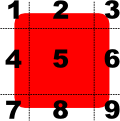
\includegraphics[width=0.2\textwidth]{figures/imgCut}
\caption{{\label{fig:cut}}Diagram ilustrující rozřezání obrázku pomocí elementu \textit{ScaledImage} \cite{bib:borderedImage}.}
\end{center}
\end{figure*}
\begin{description}
\item
\item[Seznam atributů:] ~
\begin{description}
\item[leftBorder] - hodnota udávající vzdálenost pravého řezu od pravého okraje v souřadnicích obrázku. (typ \textit{int})
\item[rightBorder] - hodnota udávající vzdálenost levého řezu od levého okraje v souřadnicích obrázku. (typ \textit{int})
\item[topBorder] - hodnota udávající vzdálenost horního řezu od horního okraje v souřadnicích obrázku. (typ \textit{int})
\item[bottomBorder] - hodnota udávající vzdálenost spodního řezu od spodního okraje v~souřadnicích obrázku. (typ \textit{int})
\item[všechny atributy z typu \textit{Image}]
\end{description}
\item[Seznam funkcí pro obsluhu událostí:] ~
\begin{description}
\item[všechny funkce z typu \textit{Image}]
\end{description}
\end{description}

\subsubsection{\textit{Text}}
Grafický element sloužící pro vykreslení textu o definovaných parametrech.\\
\begin{description}
\item[Seznam atributů:] ~
\begin{description}
\item[text] - vykreslovaný řetězec. (typ \textit{string})
\item[textColor] - barva písma. (typ \textit{Color})
\item[font] - styl písma. (typ \textit{Font})
\item[všechny atributy z typu \textit{Element}]
\end{description}
\item[Seznam funkcí pro obsluhu událostí:] ~
\begin{description}
\item[všechny funkce z typu \textit{Element}]
\end{description}
\end{description}

\subsection{\textit{Hodnotové typy}}
Některá data používaná elementy jsou sloučena do struktur, aby bylo možné s nimi manipulovat najednou. K tomuto účelu je vytvořeno několik hodnotových typů.
\subsubsection{\textit{Font}}
Datový typ, jenž slouží pro uchování údajů o stylu písma.\\
\begin{description}
\item[Seznam atributů:] ~
\begin{description}
\item[family] - název písma. (typ \textit{string})
\item[size] - velikost. (typ \textit{int})
\end{description}
\end{description}

\subsubsection{\textit{Img}}
Tato datová struktura slouží k uchování dat cesty pro načtení obrázku ze souboru.\\
\begin{description}
\item[Seznam atributů:] ~
\begin{description}
\item[src] - cesta k obrázku. (typ \textit{string})
\end{description}
\end{description}

\subsubsection{\textit{Color}}
Tato struktura slouží pro uchování údajů o barvě prostřednictvím hodnot pro červený, zelený a modrý kanál.\\
\begin{description}
\item[Seznam atributů:] ~
\begin{description}
\item[red] - hodnota červeného barevného kanálu. (typ \textit{float})
\item[green] - hodnota zeleného barevného kanálu. (typ \textit{float})
\item[blue] - hodnota modrého barevného kanálu. (typ \textit{float})
\end{description}
\end{description}



\end{document}
